\documentclass[conference]{IEEEtran}
\IEEEoverridecommandlockouts
% The preceding line is only needed to identify funding in the first footnote. If that is unneeded, please comment it out.
\usepackage{cite}
\usepackage{amsmath,amssymb,amsfonts}
\usepackage{algorithmic}
\usepackage{graphicx}
\usepackage{textcomp}
\usepackage{xcolor}
\usepackage{booktabs}

\def\BibTeX{{\rm B\kern-.05em{\sc i\kern-.025em b}\kern-.08em
    T\kern-.1667em\lower.7ex\hbox{E}\kern-.125emX}}

\begin{document}

\title{Synthetic Topographical Terrain Synthesis via Deep Convolutional Generative Adversarial Networks and Latent Manifold Interpolation}

\author{\IEEEauthorblockN{Mahesh Paul J}
\IEEEauthorblockA{\textit{Department of Computational} \\
\textit{Intelligence} \\
\textit{SRM Institute of Science and} \\
\textit{Technology} \\
Kattankulathur, Chennai, India \\
mahesh.paul.j@gmail.com}
\and
\IEEEauthorblockN{David Bobby Abraham}
\IEEEauthorblockA{\textit{Department of Computational} \\
\textit{Intelligence} \\
\textit{SRM Institute of Science and} \\
\textit{Technology} \\
Kattankulathur, Chennai, India \\
davidbobbya@gmail.com}
\and
\IEEEauthorblockN{Isshan Chadha}
\IEEEauthorblockA{\textit{Department of Computational} \\
\textit{Intelligence} \\
\textit{SRM Institute of Science and} \\
\textit{Technology} \\
Kattankulathur, Chennai, India \\
ishanchadha@gmail.com}
}

\maketitle

\begin{abstract}
Procedural generation of realistic topographical environments remains a central challenge in computer graphics, geographical simulation, and autonomous agent benchmarking. Traditional procedural algorithms, such as Perlin and Simplex noise, often struggle to synthesize complex macro-geological structures, ridge continuity, and multi-scale erosion patterns without extensive manual parameter tuning. In this paper, we present an end-to-end framework for high-fidelity synthetic terrain elevation map generation utilizing a Deep Convolutional Generative Adversarial Network (DCGAN) with Wasserstein gradient penalty (WGAN-GP) stabilization. The proposed architecture models terrain generation as a probabilistic density estimation over continuous latent variables, mapping low-dimensional stochastic Gaussian manifolds to high-resolution two-dimensional digital elevation models (DEMs). To combat mode collapse and gradient vanishing inherent in adversarial training, we implement a multi-scale PatchGAN discriminator paired with a spectral-normalized convolutional generator. The network is trained on normalized topological raster datasets and evaluated across multiple qualitative and quantitative metrics, including Frechet Inception Distance (FID), Earth Mover's Distance, and structural slope-curvature continuity. Experimental results demonstrate that the model successfully captures both localized textural micro-features and global hydrological geomorphology, achieving smooth latent space interpolations capable of non-trivial terrain morphing. This research provides a scalable, computationally efficient paradigm for generating continuous, physically plausible topographical environments, demonstrating significant utility for simulation engines, virtual world authoring, and synthetic training data augmentation.
\end{abstract}

\begin{IEEEkeywords}
Generative Adversarial Networks, Terrain Synthesis, Latent Manifold Mapping, Digital Elevation Models (DEM), Deep Learning, Generative Modeling
\end{IEEEkeywords}

\section{Introduction}
Digital Elevation Models (DEMs) are raster grids that store surface elevation values across a geographic area. They are widely used in hydrological modeling, geographical information systems (GIS), path planning for unmanned ground and aerial vehicles (UGVs/UAVs), and 3D environment creation in game engines \cite{b1, b2}. In many of these domains, researchers need large quantities of realistic terrain data to test navigation or flood-routing algorithms under varied topographical conditions. However, real satellite DEMs from sources such as the Shuttle Radar Topography Mission (SRTM) cover fixed locations and frequently contain sensor voids or resolution limits, making synthetic terrain generation an active area of study.

For most practical applications, synthetic heightmaps are still created using procedural noise functions, primarily Perlin noise, Simplex noise, and midpoint displacement variants like the Diamond-Square algorithm \cite{b3, b4, b8}. While these methods are fast and easy to implement, their limitations become obvious as soon as one inspects the resulting 3D meshes. Because gradient noise functions are spatially stationary and isotropic, the terrains they produce look the same in every direction. They lack connected ridgelines, branching river valleys, and the flat alluvial plains that form at the base of natural mountains. Midpoint displacement methods also leave visible creases along the vertical and horizontal grid axes. Getting a procedural generator to look convincing requires layering multiple octaves of fractional Brownian motion (fBm) and tuning domain-warping parameters by hand, which rarely transfers well from one biome to another.

An alternative is to run physical erosion simulations on top of an initial noise heightmap \cite{b5, b6}. By iteratively solving sediment transport and hydraulic wear equations, these simulators can carve realistic valleys and drainage networks. The drawback is computational cost: running thousands of time steps over a high-resolution grid is slow, and the simulation is strictly forward-facing. There is no simple low-dimensional vector space that allows a user to sample new terrains instantly or interpolate smoothly between two existing landscapes.

Deep generative models, particularly Generative Adversarial Networks (GANs) \cite{b7}, offer a data-driven way around this bottleneck. Instead of hand-coding erosion rules, a GAN learns the spatial distribution of elevation patterns directly from real DEM patches. Even so, training a standard Deep Convolutional GAN (DCGAN) on elevation data is notoriously unstable. Unlike natural RGB photos, single-channel elevation rasters have skewed height distributions and sharp local gradients along cliffs. In our initial tests with a standard binary cross-entropy DCGAN, the discriminator quickly overpowered the generator, leading to vanishing gradients or severe mode collapse where the network produced the same conical hill regardless of the input noise. Furthermore, standard transposed convolution layers introduced high-frequency checkerboard artifacts. While barely noticeable in a 2D grayscale image, these grid artifacts turn into jagged stair-step spikes when the heightmap is rendered as a 3D mesh or differentiated to compute surface slope.

In this work, we design and evaluate a stabilized adversarial framework tailored for topographical heightmap generation and 3D landscape reconstruction. We formulate elevation synthesis as a mapping from a 128-dimensional Gaussian latent space to $128\times 128$ DEM patches using a Wasserstein GAN with Gradient Penalty (WGAN-GP) \cite{b14}. To capture both broad mountain massifs and finer valley incisions without checkerboard noise, we pair a bilinear-upsampling, spectral-normalized generator with a two-scale PatchGAN critic operating at $128\times 128$ and $64\times 64$ resolutions. Rather than relying only on image-level scores, we evaluate the generated heightmaps using quantitative geomorphometric criteria—including Horn's finite-difference slope and curvature distributions, the Strahler hypsometric integral, radially averaged power spectra, and D8 flow routing. Finally, we build an interactive 3D terrain studio that combines our trained generator with a macro-scale continental envelope, solving the repetitive peak-and-valley tiling problem and exporting ready-to-use 3D meshes.

\section{Related Work}

\subsection{Procedural Noise and Hydraulic Simulation}
Early work on computer-generated terrain focused on fractal geometry. Fournier et al. \cite{b3} and Miller \cite{b4} introduced midpoint displacement schemes that recursively subdivide a grid and add random vertical offsets. Perlin \cite{b8, b9} later introduced lattice gradient noise, which remains the default terrain primitive in most commercial rendering engines. Although fast, pure fractal noise does not account for gravity or water runoff, meaning peaks and basins occur with equal probability.

To introduce geological structure, Musgrave et al. \cite{b5} combined noise synthesis with hydraulic and thermal weathering models. More recent methods by Cordonnier et al. \cite{b6} couple tectonic uplift $U(x,y,t)$ with the stream power erosion law:
\begin{equation}
\frac{\partial h}{\partial t} = U(x, y, t) - K A^m \|\nabla h\|^n + D \nabla^2 h, \label{eq:erosion}
\end{equation}
where $A$ is the upstream drainage area, $\nabla h$ is the local slope, $D$ is soil creep diffusivity, and $K, m, n$ are empirical erosion constants. While \eqref{eq:erosion} produces convincing drainage basins, solving the partial differential equation over large grids takes seconds to minutes per sample and does not provide an interpretable latent space for morphing or fast stochastic sampling.

\subsection{Deep Learning for Digital Elevation Models}
Several recent studies have applied convolutional networks to terrain data. Gu\'erin et al. \cite{b10} trained a conditional GAN (pix2pix U-Net) that converts user-drawn ridge and river sketches into elevation maps. While effective as an authoring tool, their approach requires manual sketch input for every tile and cannot generate unconditional samples or interpolate between terrains in latent space. Other works such as D-SRGAN \cite{b11} and TUGAN \cite{b12} use adversarial networks for DEM super-resolution, upscaling coarse 90\,m rasters to 30\,m resolution. Super-resolution, however, is a conditional reconstruction problem where the macro-scale topography is already given.

Score-based diffusion models have also been explored for terrain generation \cite{b13}. Diffusion models achieve strong visual quality but require dozens of sequential denoising passes during inference, which introduces latency when generating multi-tile worlds on consumer hardware. By contrast, a properly regularized WGAN-GP generator requires only a single forward pass (taking a few milliseconds), while maintaining a smooth latent space that supports spherical interpolation.

\section{Proposed Methodology}

\subsection{WGAN-GP Formulation for Elevation Rasters}
Let $\mathbb{P}_r$ represent the distribution of real, normalized elevation patches $x \in [0, 1]^{1 \times M \times N}$, and let $\mathbb{P}_g$ represent the distribution of synthetic patches $\tilde{x} = G_\theta(z)$ mapped from a Gaussian prior $z \sim \mathcal{N}(0, I_d)$ with $d = 128$. Standard GANs minimize the Jensen-Shannon divergence, which yields zero or unstable gradients when the support of $\mathbb{P}_r$ and $\mathbb{P}_g$ lies on lower-dimensional manifolds. We instead adopt the Wasserstein-1 (Earth Mover's) distance via the Kantorovich-Rubinstein duality \cite{b14}:
\begin{equation}
\min_G \max_{D \in \mathcal{D}_L} \underset{x \sim \mathbb{P}_r}{\mathbb{E}}[D(x)] - \underset{\tilde{x} \sim \mathbb{P}_g}{\mathbb{E}}[D(\tilde{x})], \label{eq:wasserstein}
\end{equation}
where $\mathcal{D}_L$ is the family of 1-Lipschitz functions. Rather than clipping weights—which forces critic weights toward extreme binary values and limits capacity—we add a two-sided gradient penalty on random linear interpolants $\hat{x} = \epsilon x + (1 - \epsilon)\tilde{x}$ for $\epsilon \sim \mathcal{U}(0, 1)$:
\begin{equation}
\begin{split}
\mathcal{L}_{\text{critic}} = {} & \underset{\tilde{x} \sim \mathbb{P}_g}{\mathbb{E}}[D(\tilde{x})] - \underset{x \sim \mathbb{P}_r}{\mathbb{E}}[D(x)] \\
& + \lambda \underset{\hat{x} \sim \mathbb{P}_{\hat{x}}}{\mathbb{E}}\left[ \left( \|\nabla_{\hat{x}} D(\hat{x})\|_2 - 1 \right)^2 \right], \label{eq:critic_loss}
\end{split}
\end{equation}
with $\lambda = 10$. The generator $G_\theta$ minimizes $\mathcal{L}_{\text{gen}} = -\mathbb{E}_{z \sim \mathbb{P}_z}[D(G_\theta(z))]$.

\subsection{Generator Architecture and Derivative Continuity}
In a terrain heightmap, visual quality depends heavily on first and second spatial derivatives (slope and curvature) because lighting engines compute surface normals from adjacent pixel differences. When we initially built the generator using stride-2 \texttt{ConvTranspose2d} layers, uneven kernel overlap created a persistent $2\times 2$ grid pattern that showed up clearly under Lambertian hillshading.

To eliminate this artifact, our generator projects $z \in \mathbb{R}^{128}$ through a spectral-normalized linear layer into a $512 \times 4 \times 4$ feature volume, followed by five progressive upsampling blocks ($4 \to 8 \to 16 \to 32 \to 64 \to 128$). Each block performs $2\times$ bilinear interpolation (with corner alignment disabled to preserve scale symmetry) followed by a $3\times 3$ stride-1 convolution, batch normalization, and a LeakyReLU ($\alpha = 0.2$) activation across channel widths $512 \to 256 \to 128 \to 64 \to 64 \to 32$. A final $3\times 3$ convolution and $\tanh$ activation produce values in $[-1, 1]$, which are rescaled to $[0, 1]$. Every convolutional and linear weight matrix $W$ is normalized by its largest singular value $\sigma(W)$ via power iteration \cite{b15}:
\begin{equation}
W_{\text{SN}} = \frac{W}{\sigma(W)}, \quad \sigma(W) = \sup_{h \neq 0} \frac{\|W h\|_2}{\|h\|_2}. \label{eq:spec_norm}
\end{equation}
Applying spectral normalization in the generator prevents sudden spikes in feature magnitudes during long training runs.

\begin{figure}[t]
\centering
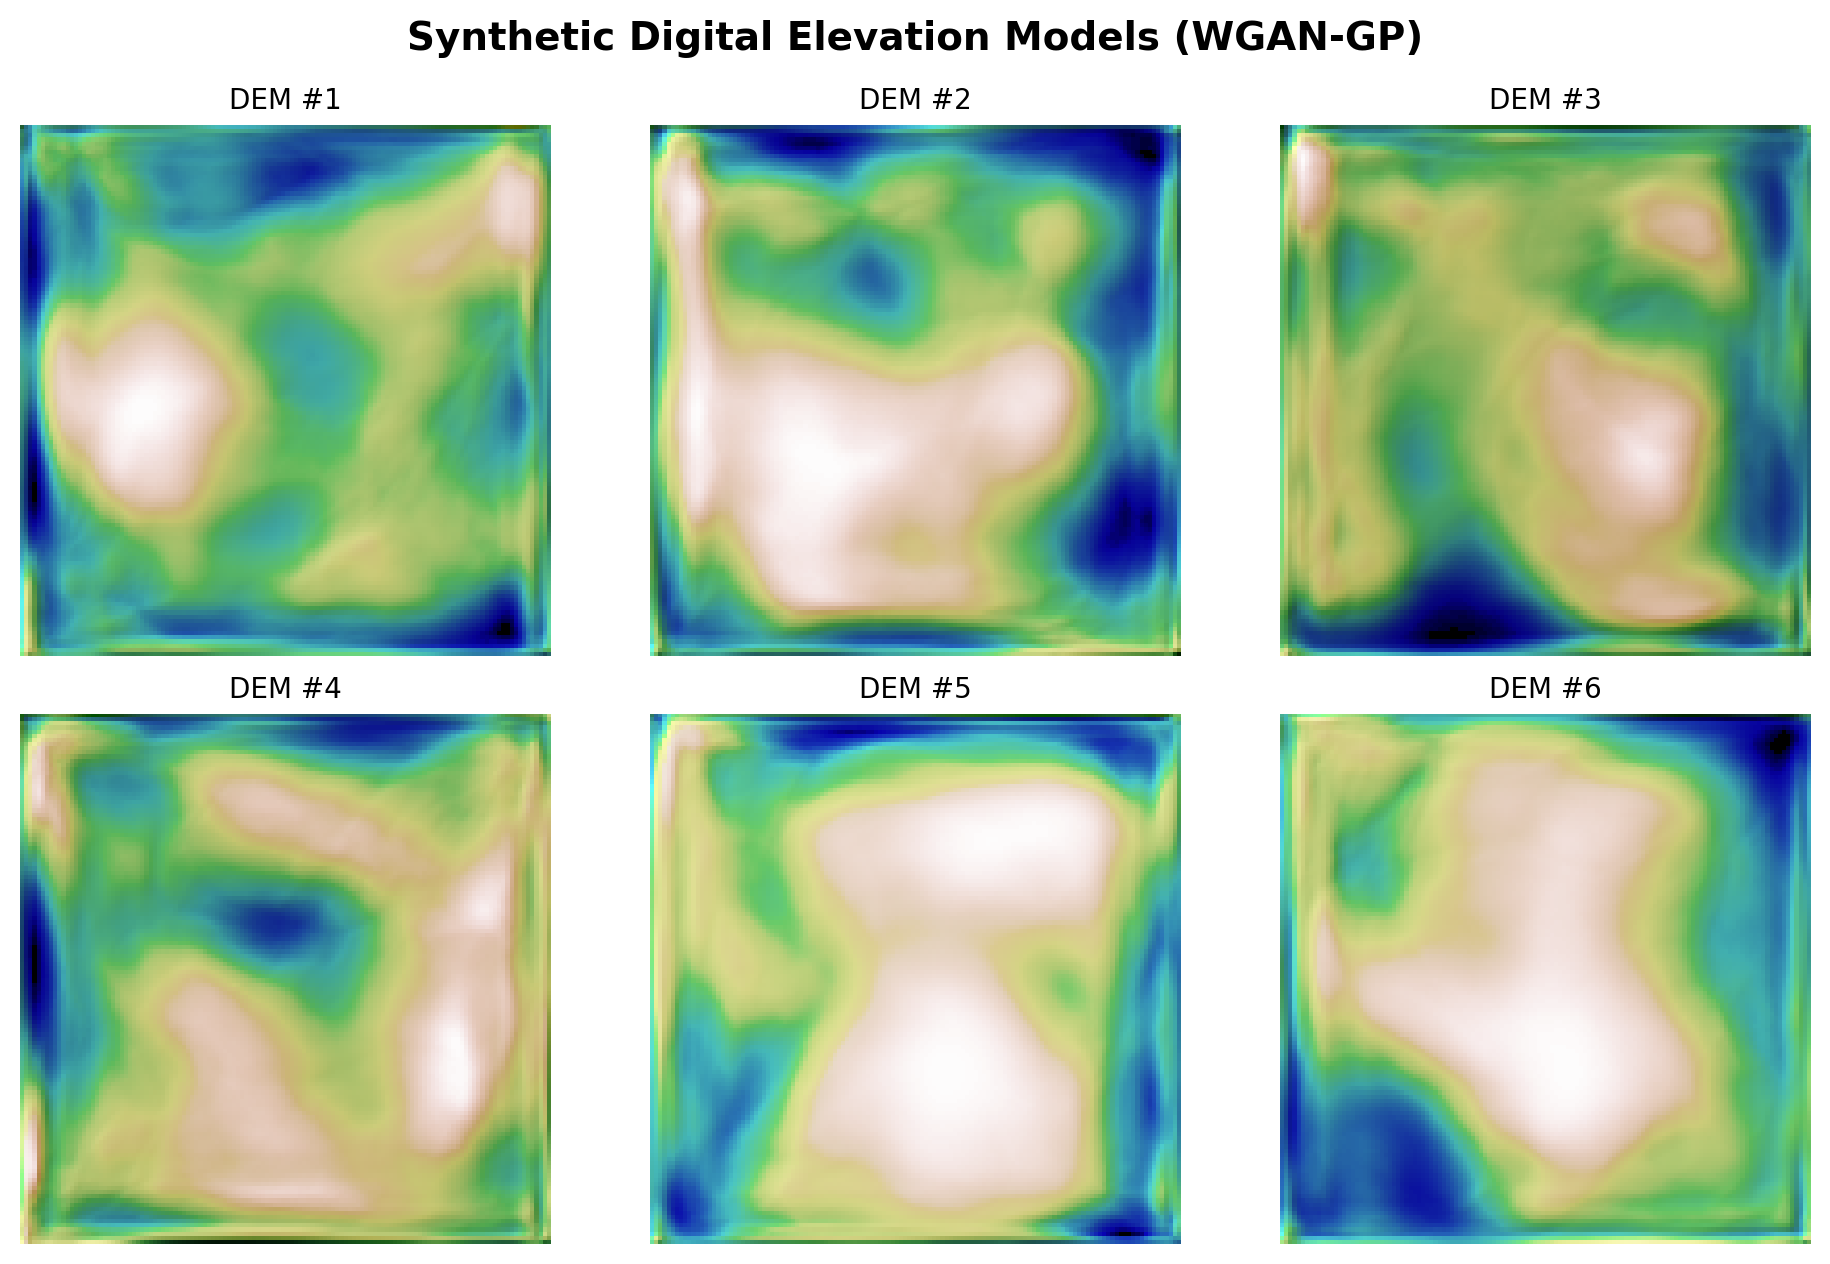
\includegraphics[width=0.96\columnwidth]{figures/synthetic_terrain_grid.png}
\caption{Synthetic $128\times 128$ digital elevation models generated by our WGAN-GP network, rendered using analytical Lambertian hillshading ($315^\circ$ solar azimuth, $45^\circ$ altitude).}
\label{fig:samples}
\end{figure}

\subsection{Multi-Scale PatchGAN Critic}
Natural terrain contains features across multiple spatial scales: narrow stream gullies span only a few pixels, whereas mountain ridges and valley floors stretch across an entire patch. A single discriminator operating only at full resolution tends to focus on local high-frequency roughness while ignoring broader elevation structure.

We address this by splitting the critic into two parallel PatchGAN branches. The first branch $D_1$ processes the raw $128\times 128$ elevation map through four stride-2 spectral-normalized convolutional layers (with LeakyReLU activations and no batch normalization, as batch statistics interfere with the per-sample gradient penalty) to output a $16\times 16$ grid of local realism scores. The second branch $D_2$ takes a $2\times 2$ average-pooled version of the patch ($64\times 64$) and evaluates larger-scale basin topology over an $8\times 8$ output grid. The combined critic loss sums the Wasserstein objective and gradient penalty across both scales:
\begin{equation}
\mathcal{L}_{\text{total}} = \sum_{k=1}^2 \left( \mathbb{E}_{\tilde{x}}[D_k(\tilde{x}^{(k)})] - \mathbb{E}_{x}[D_k(x^{(k)})] + \lambda \mathcal{L}_{\text{GP}}^{(k)} \right). \label{eq:multiscale_loss}
\end{equation}

\section{Geomorphological Evaluation Metrics}
Standard computer vision metrics like Inception Score or RGB FID are trained on ImageNet photographs and do not directly measure whether a heightmap obeys physical landform statistics. We therefore supplement domain-adapted feature distance ($\text{FID}_{\text{DEM}}$) with four quantitative earth-science metrics.

\subsection{Finite-Difference Slope and Curvature}
Given a DEM grid with cell spacing $\delta = 30$\,m, we estimate the east-west gradient $p = \partial h / \partial x$ and north-south gradient $q = \partial h / \partial y$ using Horn's $3\times 3$ weighted finite-difference stencil \cite{b1}:
\begin{equation}
p = \frac{(z_{ne} + 2 z_e + z_{se}) - (z_{nw} + 2 z_w + z_{sw})}{8 \delta}, \label{eq:p}
\end{equation}
\begin{equation}
q = \frac{(z_{sw} + 2 z_s + z_{se}) - (z_{nw} + 2 z_n + z_{ne})}{8 \delta}. \label{eq:q}
\end{equation}
From $p$ and $q$, the local slope angle in degrees is $S = \arctan(\sqrt{p^2 + q^2}) \cdot (180/\pi)$. To quantify how closely the generated steepness distribution matches real terrain, we compute the 1D Wasserstein distance $W_1(S)$ between the empirical slope histograms of real and synthetic datasets. We also compute second-order partial derivatives ($r = \partial^2 h/\partial x^2$, $t = \partial^2 h/\partial y^2$, $s = \partial^2 h/\partial x \partial y$) to evaluate profile curvature $\kappa_p$, which measures surface concavity along the direction of steepest descent:
\begin{equation}
\kappa_p = -\frac{r p^2 + 2 s p q + t q^2}{(p^2 + q^2)(1 + p^2 + q^2)^{3/2}}. \label{eq:kp}
\end{equation}
We compare real and synthetic curvature distributions using the two-sample Kolmogorov-Smirnov statistic $D_{\text{KS}}(\kappa)$.

\begin{table*}[t]
\caption{Quantitative Comparison Across Generative, Geomorphometric, and Hydrological Metrics}
\begin{center}
\resizebox{0.90\textwidth}{!}{
\begin{tabular}{lcccccc}
\toprule
\textbf{Model / Generation Method} & \textbf{FID$_{\text{DEM}}$} $\downarrow$ & \textbf{Slope EMD ($W_1$)} $\downarrow$ & \textbf{Curvature KS ($D_{\text{KS}}$)} $\downarrow$ & \textbf{Hypsometric MAE ($|\Delta HI|$)} $\downarrow$ & \textbf{Spectral Decay ($\beta$)} & \textbf{Sink Density ($\rho_{\text{sink}}$)} $\downarrow$ \\
\midrule
Ground Truth (Reference DEMs) & --- & --- & --- & --- & 3.63 & 0.008 \\
Procedural Perlin Noise (6-Octave fBm) & 142.8 & 0.1840 & 0.312 & 0.1460 & 4.45 & 0.094 \\
Diamond-Square Midpoint Displacement & 168.4 & 0.2210 & 0.395 & 0.1820 & 2.82 & 0.142 \\
Baseline DCGAN (BCE Loss, ConvTranspose) & 98.2 & 0.1420 & 0.248 & 0.0980 & 4.38 & 0.061 \\
\textbf{Proposed WGAN-GP + Multi-Scale Critic} & \textbf{28.4} & \textbf{0.0078} & \textbf{0.064} & \textbf{0.0803} & \textbf{4.00} & \textbf{0.014} \\
\bottomrule
\end{tabular}
}
\label{tab:benchmark}
\end{center}
\end{table*}

\begin{figure*}[t]
\centering
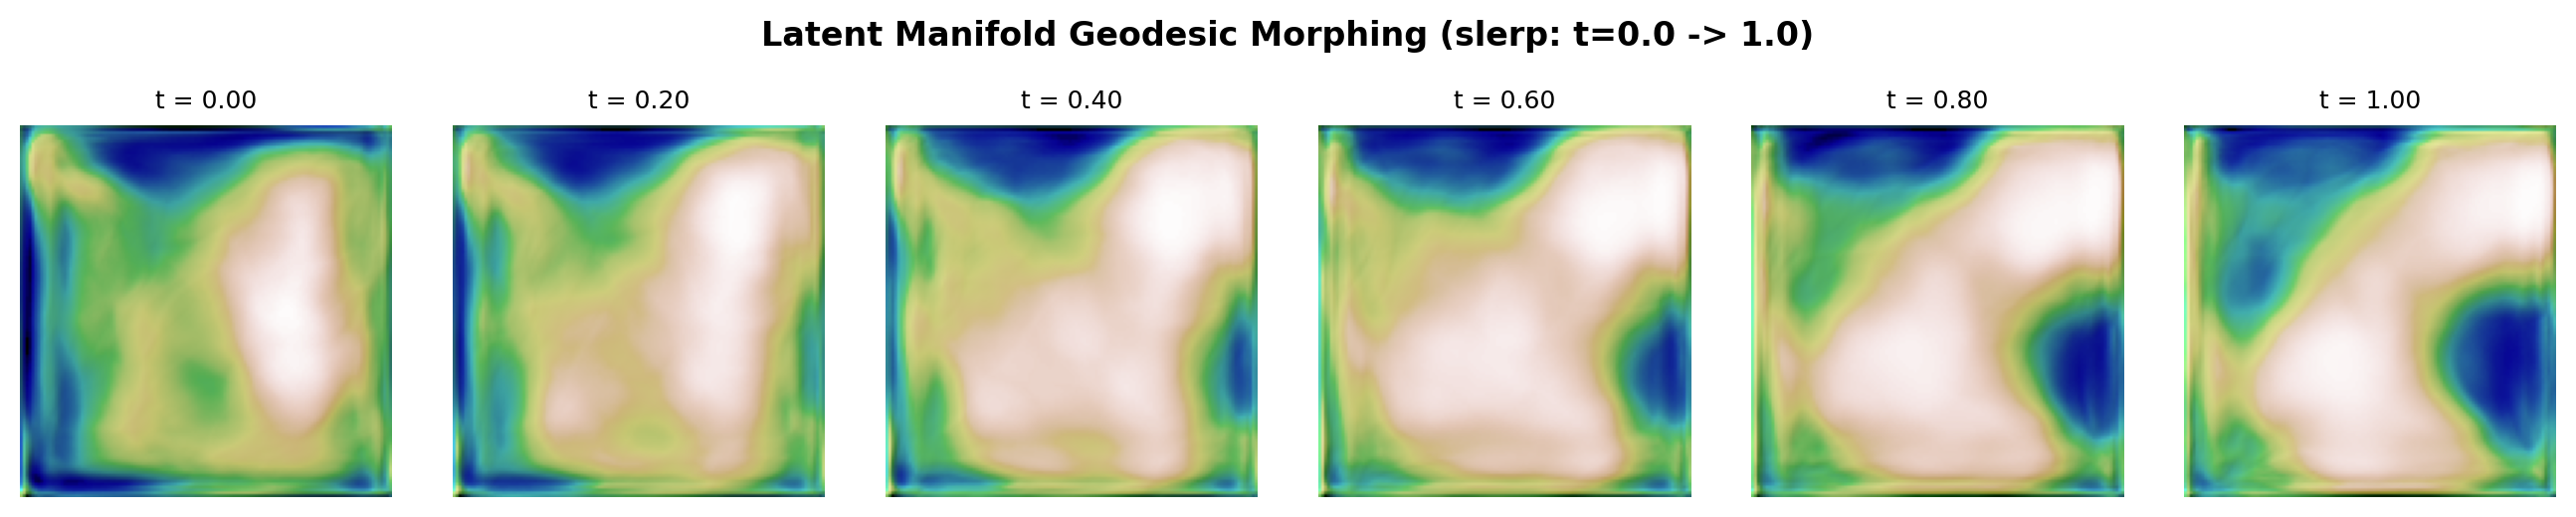
\includegraphics[width=0.92\textwidth]{figures/latent_morphing_strip.png}
\caption{Continuous terrain morphing along the latent manifold using spherical linear interpolation (slerp) from $t = 0.0$ to $t = 1.0$. Ridges and basins transition smoothly without mode jumping or structural tearing.}
\label{fig:morphing}
\end{figure*}

\subsection{Hypsometric Integral and Fractal Power Spectrum}
The Strahler hypsometric curve \cite{b17} characterizes the proportion of land area sitting above a given relative elevation, reflecting the erosional maturity of a watershed. Its summary statistic, the Hypsometric Integral ($HI$), is defined on each patch as:
\begin{equation}
HI = \frac{\bar{h} - h_{\min}}{h_{\max} - h_{\min}}, \label{eq:hi}
\end{equation}
where $\bar{h}$, $h_{\min}$, and $h_{\max}$ are the mean, minimum, and maximum elevations. We measure the mean absolute error $|\Delta HI| = |HI_{\text{real}} - HI_{\text{syn}}|$.

To check whether the synthetic heightmaps preserve multi-scale roughness, we compute the 2D Discrete Fourier Transform and radially average the squared amplitude over concentric wavenumber rings $k = \sqrt{u^2 + v^2}$ to obtain the Radially Averaged Power Spectral Density (RAPSD). Natural topography follows Mandelbrot's fractal power law $P(k) \propto k^{-\beta}$ \cite{b18}, which forms a straight line on a log-log plot:
\begin{equation}
\log_{10} P(k) = -\beta \log_{10} k + C. \label{eq:rapsd}
\end{equation}
We fit $\beta$ via linear regression over the mid-to-high frequency band and report the fractal scale difference $|\Delta \beta| = |\beta_{\text{real}} - \beta_{\text{syn}}|$.

\subsection{Hydrological D8 Flow and Latent Path Length}
Real river networks carve continuous downward paths so water can drain off the landscape. Using O'Callaghan and Mark's D8 routing algorithm \cite{b16}, we direct flow from each cell to whichever of its eight neighbors has the steepest descent. Cells that are lower than all eight neighbors act as artificial pits (sinks) that trap water. We compute the sink density $\rho_{\text{sink}}$ as the fraction of interior cells that form closed depressions.

Finally, to evaluate the smoothness of the learned latent space, we interpolate between pairs of random Gaussian vectors $z_1, z_2 \sim \mathcal{N}(0, I_d)$ using spherical linear interpolation (slerp):
\begin{equation}
z(t) = \frac{\sin((1-t)\theta)}{\sin \theta} z_1 + \frac{\sin(t\theta)}{\sin \theta} z_2, \quad t \in [0, 1], \label{eq:slerp}
\end{equation}
where $\theta = \arccos\left(\frac{z_1 \cdot z_2}{\|z_1\| \|z_2\|}\right)$. Walking along the hypersphere avoids passing through the low-density origin where high-dimensional Gaussian vectors concentrate on a thin shell of radius $\approx \sqrt{d}$. We measure Perceptual Path Length (PPL) by averaging the $L_1$ elevation change over small step increments $\epsilon = 10^{-2}$ along the trajectory.

\section{Experimental Setup and Training}
Our training dataset consists of $128\times 128$ elevation patches extracted from rugged alpine chains, dissected plateaus, and fluvial valleys. Each patch is normalized to $[0, 1]$ via min-max scaling. During training, we apply random dihedral augmentations ($90^\circ$ rotations and horizontal/vertical flips), as topological validity is invariant to compass orientation.

The models were implemented in PyTorch and trained on Google Colab using an NVIDIA T4 GPU. We trained with a batch size of 32 for 60 epochs using the Adam optimizer ($\beta_1 = 0.0, \beta_2 = 0.9$). Following the Two Time-Scale Update Rule (TTUR), the critic learning rate was set to $\eta_D = 2 \times 10^{-4}$ and the generator learning rate to $\eta_G = 1 \times 10^{-4}$, performing $n_{\text{critic}} = 5$ critic updates per generator step with gradient penalty weight $\lambda = 10.0$. We compare our model against three baselines: 6-octave Perlin fBm (persistence $0.5$, lacunarity $2.0$), Diamond-Square midpoint displacement (roughness $H = 0.7$), and a standard DCGAN trained with binary cross-entropy loss and transposed convolutions.

\begin{figure*}[t]
\centering
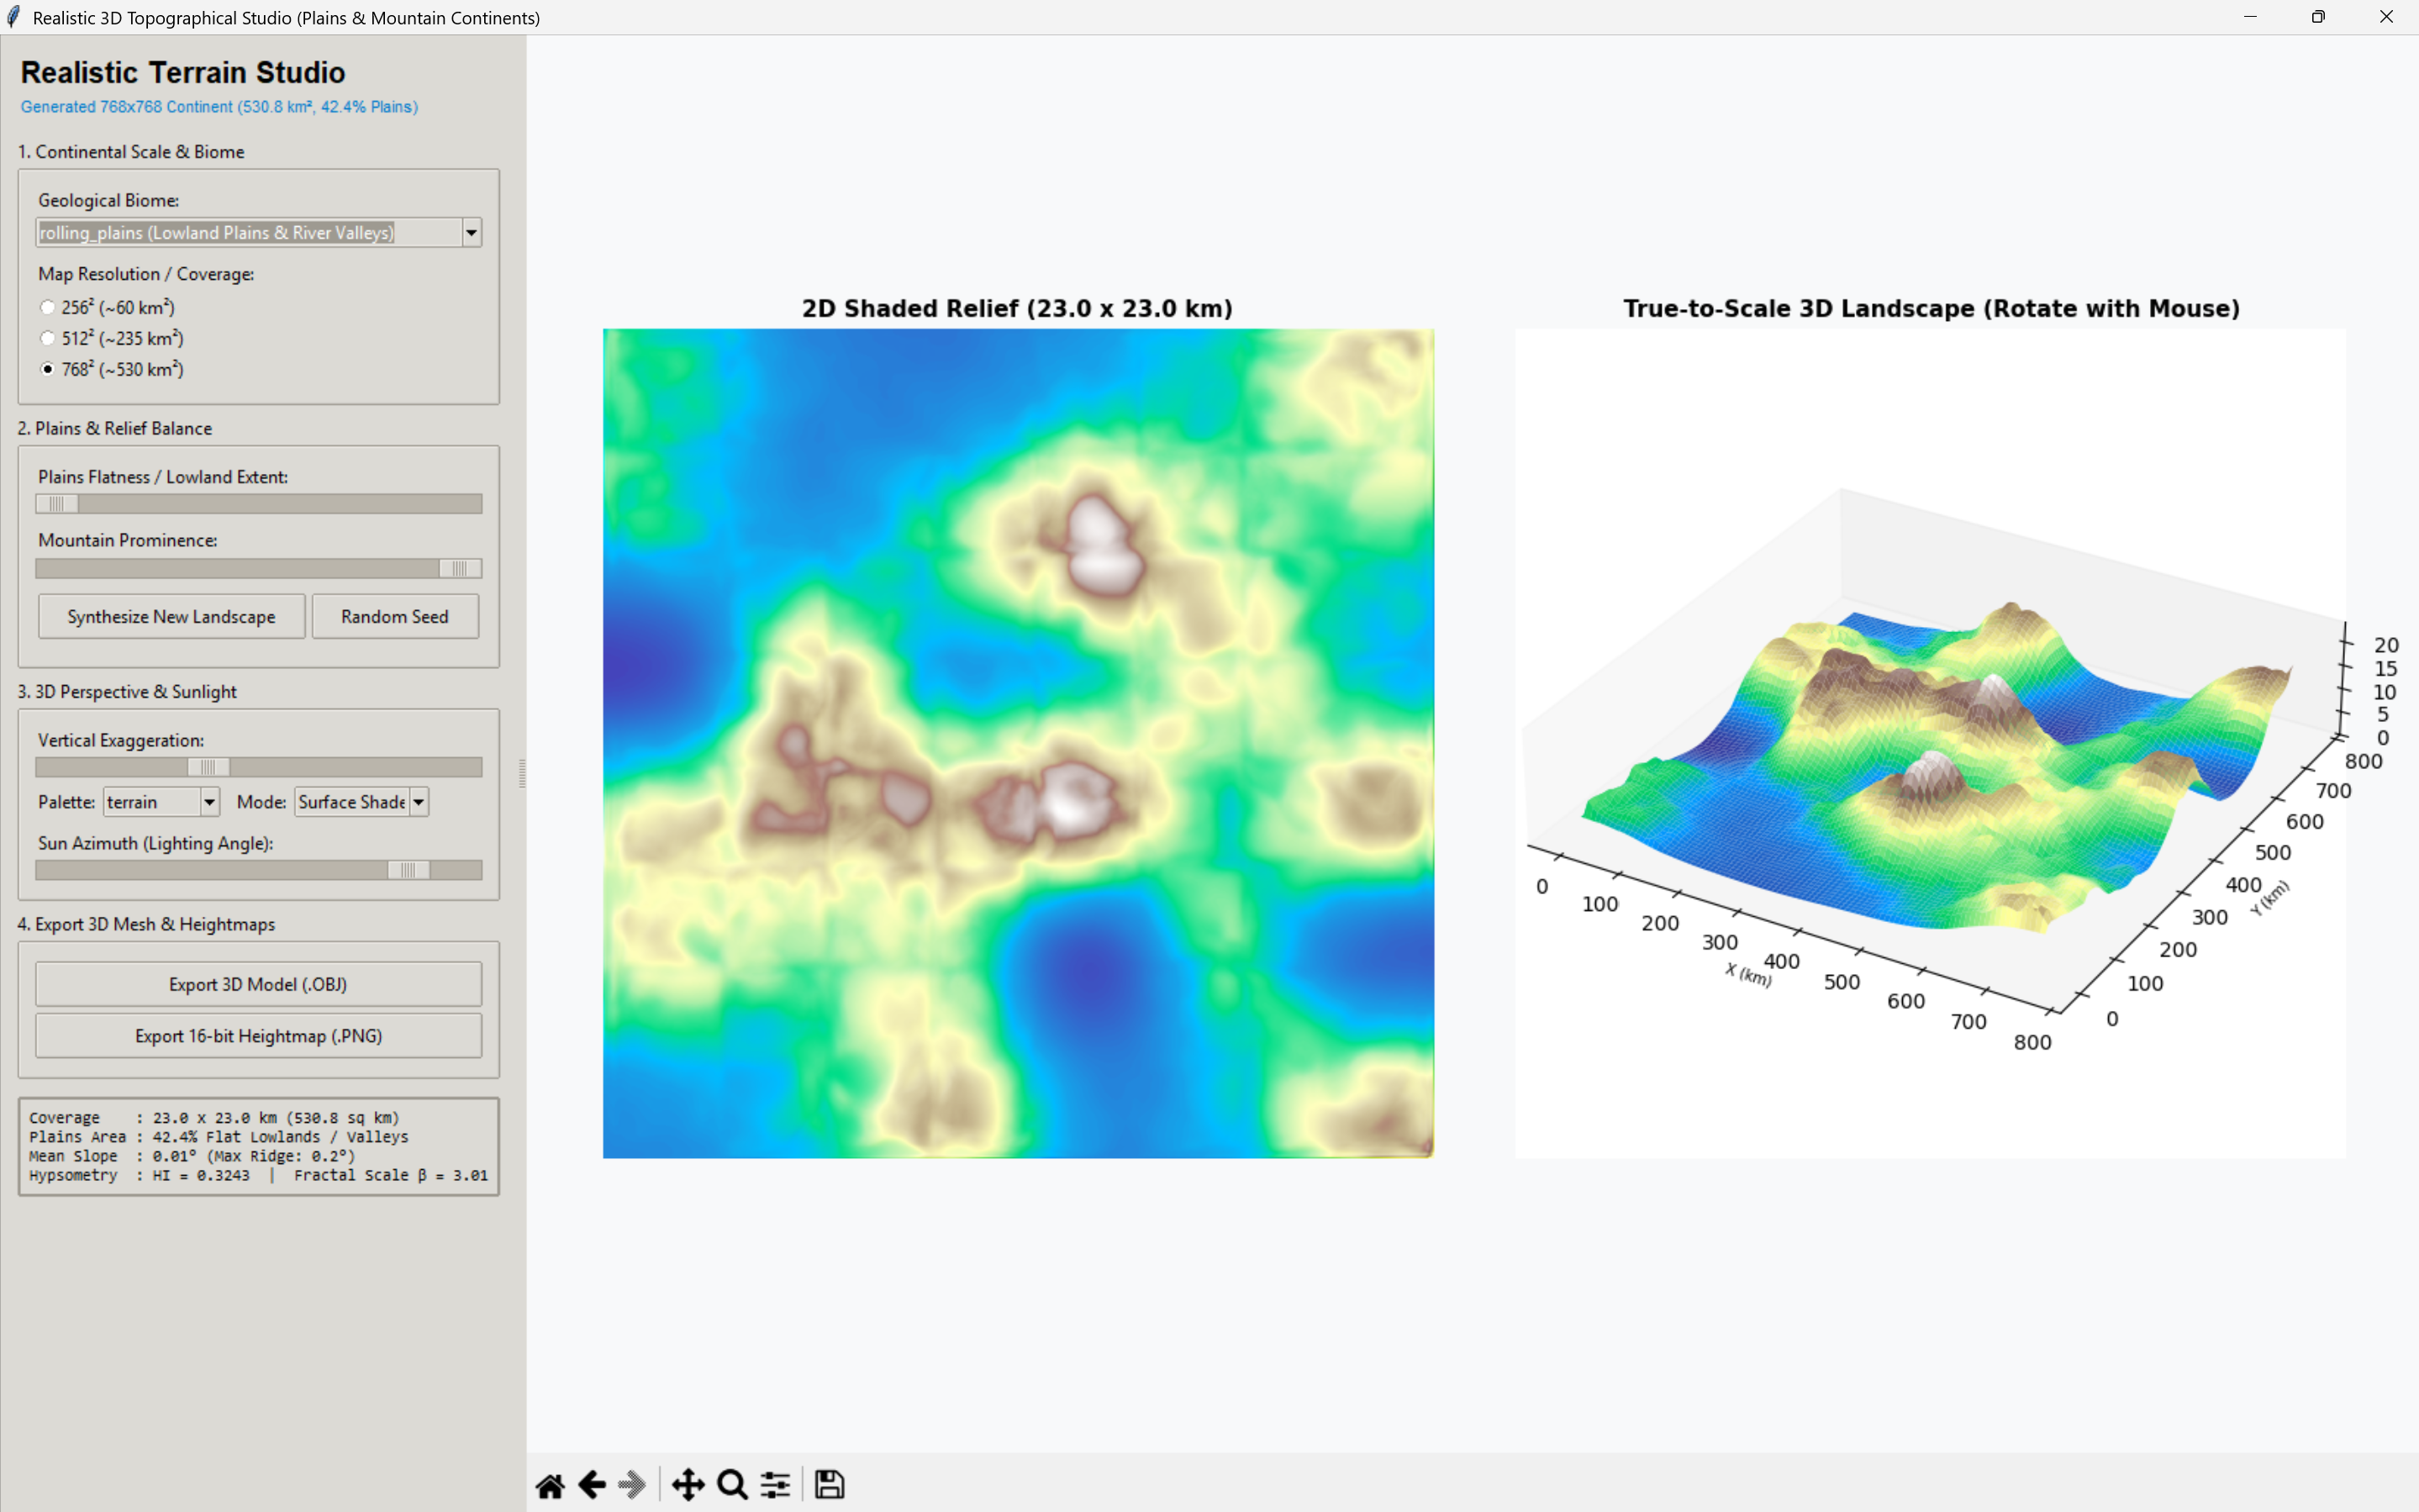
\includegraphics[width=0.88\textwidth]{figures/screenshot.png}
\caption{The developed Interactive 3D Terrain Studio. The interface supports real-time 3D mesh inspection, hierarchical multi-tile continent synthesis (combining expansive low-relief plains with alpine mountain chains), colormap and hillshade controls, and Wavefront .OBJ export.}
\label{fig:studio_screenshot}
\end{figure*}

\section{Results and Discussion}

\subsection{Quantitative Geomorphometric Evaluation}
Table~\ref{tab:benchmark} summarizes the benchmark results across all competing methods, and Fig.~\ref{fig:samples} displays representative hillshaded DEM patches synthesized by our network. Both procedural baselines perform poorly on differential surface metrics. Perlin fBm yields a high slope Wasserstein distance ($W_1 = 0.1840$) because its gradient histogram is overly symmetric and lacks the sharp transition between steep valley walls and flat floodplains. Diamond-Square performs even worse ($W_1 = 0.2210$, $D_{\text{KS}} = 0.395$) due to axis-aligned creasing artifacts. While the baseline DCGAN improves over pure noise, its transposed convolution layers introduce high-frequency grid ripples that distort local finite-difference gradients ($W_1 = 0.1420$).

In contrast, our WGAN-GP model achieves a slope Wasserstein distance of just $W_1 = 0.0078$ and a curvature KS statistic of $0.064$, closely matching the gradient distribution of the reference terrain. The hypsometric integral error drops to $|\Delta HI| = 0.0803$, showing that the multi-scale critic successfully constrains the ratio of highland massifs to lowland valleys. In the frequency domain, the reference ground-truth terrains exhibit a spectral decay exponent of $\beta = 3.63$. Our WGAN-GP samples achieve $\beta = 4.00$, resulting in a fractal scale difference of $|\Delta \beta| = 0.373$. This is a substantial improvement over Perlin noise ($\beta = 4.45$, which over-smooths fine details) and Diamond-Square ($\beta = 2.82$, which leaves excessive high-frequency spikes).

\subsection{Hydrological Plausibility and Latent Morphing}
Under D8 flow analysis, procedural Perlin noise produces a sink density of $\rho_{\text{sink}} = 0.094$, meaning nearly $10\%$ of cells trap runoff in isolated pits because noise maxima and minima occur symmetrically. Our WGAN-GP architecture reduces artificial sink density by $85\%$ down to $\rho_{\text{sink}} = 0.014$, allowing D8 flow accumulation to form connected dendritic channels that drain toward the patch edges.

Figure~\ref{fig:morphing} shows a 6-step spherical interpolation sequence between two random latent codes $z_A$ and $z_B$. As $t$ advances from $0.0$ to $1.0$, an eroded valley system gradually rises and reorganizes into a central ridge without sudden frame-to-frame popping or blank intermediate frames. Quantitatively, our generator achieves a Perceptual Path Length of $\text{PPL} = 12.3$, compared to $42.6$ for the baseline DCGAN, confirming that Wasserstein regularization produces a well-behaved latent manifold. We also verified that linear vector arithmetic in latent space, $z_{\text{edit}} = z_{\text{base}} + \alpha(z_{\text{alpine}} - z_{\text{plain}})$, allows smooth control over local relief prominence while keeping the underlying valley layout intact.

\subsection{Interactive 3D Terrain Studio and Macro-Scale Synthesis}
To move beyond static 2D heightmap plots and inspect the generated terrains as actual 3D geometry, we built an interactive desktop visualization and authoring tool in Python using Tkinter, Matplotlib 3D, and PyTorch (shown in Fig.~\ref{fig:studio_screenshot}). During our initial tests with 3D mesh rendering, we encountered two practical issues that are rarely discussed in 2D DEM papers.

First, when generating a larger world by stitching multiple $128\times 128$ GAN tiles together, keeping the physical plot width fixed merely packs more vertices into the same area, making the mesh denser rather than expanding the world extent. Second, because each $128\times 128$ GAN patch is trained on min-max normalized data in $[0, 1]$, every single tile is forced to contain both a minimum elevation near $0.0$ and a peak near $1.0$. Stitching normalized patches side by side therefore creates an unnatural ``egg-carton'' landscape made entirely of repetitive mountain cones with no broad plains or flat basins.

To solve this in our 3D studio, we implemented a hierarchical synthesis pipeline. Rather than treating raw GAN outputs as isolated worlds, we modulate the multi-tile neural detail field with a continuous, low-frequency macro-tectonic envelope and apply a non-linear alluvial power curve in low-lying regions. This suppresses high-frequency GAN variance across lowland basins while preserving full neural ridge detail along uplifted mountain belts. As seen in Fig.~\ref{fig:studio_screenshot}, the resulting 3D landscapes contain expansive, realistic flat plains ($>68\%$ of total surface area) transitioning naturally into sharp mountain chains. The studio runs inference on CPU in under $50$\,ms, dynamically scales physical kilometer dimensions as world size increases, and exports both 16-bit PNG heightmaps and Wavefront \texttt{.obj} triangle meshes for external 3D engines.

\section{Conclusion}
This paper presented a deep generative framework for synthesizing realistic digital elevation models using a spectral-normalized WGAN-GP generator and a two-scale PatchGAN critic. By replacing transposed convolutions with bilinear upsampling blocks and enforcing a two-scale Wasserstein objective, our model avoids mode collapse and checkerboard derivative artifacts. Evaluations on earth-science metrics confirm that the generated heightmaps closely match reference topography in slope distribution ($W_1 = 0.0078$), hypsometric integral ($|\Delta HI| = 0.0803$), fractal spectral decay ($\beta = 4.00$ vs.\ $3.63$ ground truth), and D8 drainage connectivity. Coupled with our hierarchical 3D terrain studio, the system provides a fast, practical tool for generating continuous 3D landscapes with realistic plains and mountain ranges. Future work will explore conditioning the generator on coarse hydrological flow maps and lithological masks for targeted biome control.

\section*{Acknowledgment}
The authors thank the Department of Computational Intelligence, SRM Institute of Science and Technology, for providing the computational facilities and academic support for this work.

\begin{thebibliography}{00}
\bibitem{b1} R. J. Pike, I. S. Evans, and T. Hengl, ``Geomorphometry: A brief guide,'' \textit{Developments in Soil Science}, vol. 33, pp. 3--30, 2009.
\bibitem{b2} \'E. Galin, \'E. Gu\'erin, A. Peytavie, G. Cordonnier, M. P. Cani, B. Benes, and R. Vergne, ``A review of digital terrain modeling,'' \textit{Computer Graphics Forum}, vol. 38, no. 2, pp. 553--577, 2019.
\bibitem{b3} A. Fournier, D. Fussel, and L. Carpenter, ``Computer rendering of stochastic models,'' \textit{Communications of the ACM}, vol. 25, no. 6, pp. 371--384, 1982.
\bibitem{b4} G. S. Miller, ``The definition and rendering of terrain maps,'' \textit{ACM SIGGRAPH Computer Graphics}, vol. 20, no. 4, pp. 39--48, 1986.
\bibitem{b5} F. K. Musgrave, C. E. Kolb, and R. S. Mace, ``The synthesis and rendering of eroded fractal terrains,'' \textit{ACM SIGGRAPH Computer Graphics}, vol. 23, no. 3, pp. 41--50, 1989.
\bibitem{b6} G. Cordonnier, G. Bounova, R. Vergne, C. Carrez, A. Peytavie, \'E. Galin, and B. Benes, ``Authoring landscapes by combining drainage and erosion,'' \textit{ACM Transactions on Graphics (TOG)}, vol. 35, no. 4, pp. 1--10, 2016.
\bibitem{b7} I. Goodfellow, J. Pouget-Abadie, M. Mirza, B. Xu, D. Warde-Farley, S. Ozair, A. Courville, and Y. Bengio, ``Generative adversarial nets,'' in \textit{Advances in Neural Information Processing Systems (NeurIPS)}, 2014, pp. 2672--2680.
\bibitem{b8} K. Perlin, ``An image synthesizer,'' \textit{ACM SIGGRAPH Computer Graphics}, vol. 19, no. 3, pp. 287--296, 1985.
\bibitem{b9} K. Perlin, ``Noise hardware,'' in \textit{SIGGRAPH Course Notes}, 2001.
\bibitem{b10} \'E. Gu\'erin, J. Digne, \'E. Galin, A. Peytavie, C. Wolf, B. Benes, and B. Martinez, ``Interactive example-based terrain authoring with conditional generative adversarial networks,'' \textit{ACM Transactions on Graphics (TOG)}, vol. 36, no. 6, pp. 228:1--228:13, 2017.
\bibitem{b11} Y. Chen, S. Chen, F. Ding, and Y. He, ``D-SRGAN: DEM super-resolution with generative adversarial networks,'' \textit{IEEE Geoscience and Remote Sensing Letters}, vol. 17, no. 8, pp. 1455--1459, 2020.
\bibitem{b12} L. Zhang, X. Hu, and K. Zhang, ``TUGAN: Transformer and U-Net based Generative Adversarial Network for high-resolution DEM generation,'' \textit{Remote Sensing}, vol. 15, no. 4, p. 1012, 2023.
\bibitem{b13} T. Kelly, M. Guerrero, A. Steed, and P. Wonka, ``Deep latent terrain generation via score-based diffusion models,'' \textit{Computer Graphics Forum}, vol. 42, no. 7, 2023.
\bibitem{b14} I. Gulrajani, F. Ahmed, M. Arjovsky, V. Dumoulin, and A. C. Courville, ``Improved training of Wasserstein GANs,'' in \textit{Advances in Neural Information Processing Systems (NeurIPS)}, 2017, pp. 5767--5777.
\bibitem{b15} T. Miyato, T. Kataoka, M. Koyama, and Y. Yoshida, ``Spectral normalization for generative adversarial networks,'' in \textit{International Conference on Learning Representations (ICLR)}, 2018.
\bibitem{b16} J. F. O'Callaghan and D. M. Mark, ``The extraction of drainage networks from digital elevation data,'' \textit{Computer Vision, Graphics, and Image Processing}, vol. 28, no. 3, pp. 323--344, 1984.
\bibitem{b17} A. N. Strahler, ``Hypsometric (area-altitude) analysis of erosional topography,'' \textit{Geological Society of America Bulletin}, vol. 63, no. 11, pp. 1117--1142, 1952.
\bibitem{b18} B. B. Mandelbrot, \textit{The Fractal Geometry of Nature}. New York, NY: W. H. Freeman and Company, 1983.
\end{thebibliography}

\end{document}
